\section{Analysis of MSVV}

\subsection{A Discretized Version of MSVV}

\begin{frame}
    \frametitle{Assumptions}
	\begin{enumerate}
        \item<1-> Each bid is small compared to the corresponding budget \mbox{(i.e., $\forall (u,v) \in E: c_{u,v} \ll b_u$}).
        \item<1-> Each bidder has a budget of $1$.
        \invisible<1->{
            \item<1-> \textcolor{orange}{OPT} exhausts the budget of each bidder.
            \item<1-> Each bidder of type $i \in \{1,...,k \}$ spends exactly $\frac{i}{k}$.
            \item<1-> All non-zero bids are equal.   
        }
	\end{enumerate}
\end{frame}

\begin{frame}
    \frametitle{Slab}
    The budget of each bidder is \textcolor{blue}{discretized} into $k$ equal parts, where $k$ is a large integer.
    \begin{definition}
        Let $i \in \{1, \dots, k \}$. \alert{Slab} $i$ is the $\left[\frac{i-1}{k}, \frac{i}{k} \right)$ portion of each bidder's budget.
    \end{definition}
    \begin{block}{Notation}
        Let $u \in U, v \in V$. Then slab($u,v$) denotes the \textcolor{blue}{currently} active slab for $u$ at the arrival of $v$. If $v$ is apparent from the context, we write slab($u$) instead.\\
        \smallskip
        Let $i \in \{1, \dots, k \}$. Then $\beta_i$ denotes the total money spent by the bidders from slab $i$ in the run of \textcolor{orange}{MSVV}.
    \end{block}
\end{frame}

\begin{frame}
    \frametitle{Assumptions}
	\begin{enumerate}
        \item<1-> $\forall (u,v) \in E: c_{u,v} \leq \frac{1}{k^2}$.
        \item<1-> Each bidder has a budget of $1$.
        \invisible<1->{
            \item<1-> \textcolor{orange}{OPT} exhausts the budget of each bidder.
            \item<1-> Each bidder of type $i \in \{1,...,k \}$ spends exactly $\frac{i}{k}$.
            \item<1-> All non-zero bids are equal.   
        }
	\end{enumerate}
\end{frame}

\begin{frame}
    \begin{block}{Notation}
        $n := |U|$
    \end{block}
    \begin{definition}
        Let $i \in \{1, \dots, k \}$. A bidder is of \alert{type} $i$ if the money spent by it \textcolor{blue}{at the end} of \textcolor{orange}{MSVV} lies in the range $\left(\frac{i-1}{k}, \frac{i}{k} \right]$.\\
        \smallskip
        By convention a bidder who spends none of its budget is assigned type $1$.
    \end{definition}
    \begin{block}{Notation}
        Let $u \in U$. Then type($u$) denotes the type of bidder $u$.\\
        \smallskip
        Let $i \in \{1, \dots, k \}$. Then $x_i$ denotes the number of bidders of type $i$ (so, $\sum_{i=1}^k x_i = n$).
    \end{block}
\end{frame}

\begin{frame}
    \frametitle{Assumptions}
	\begin{enumerate}
        \item<1-> $\forall (u,v) \in E: c_{u,v} \leq \frac{1}{k^2}$.
        \item<1-> Each bidder has a budget of $1$.
        \item<1-> \textcolor{orange}{OPT} exhausts the budget of each bidder.
        \invisible<1->{
            \item<1-> Each bidder of type $i \in \{1,...,k \}$ spends exactly $\frac{i}{k}$.
            \item<1-> All non-zero bids are equal.   
        }
	\end{enumerate}
\end{frame}

\begin{frame}
    \frametitle{Revenue Structure at the End of MSVV}
    \centering
	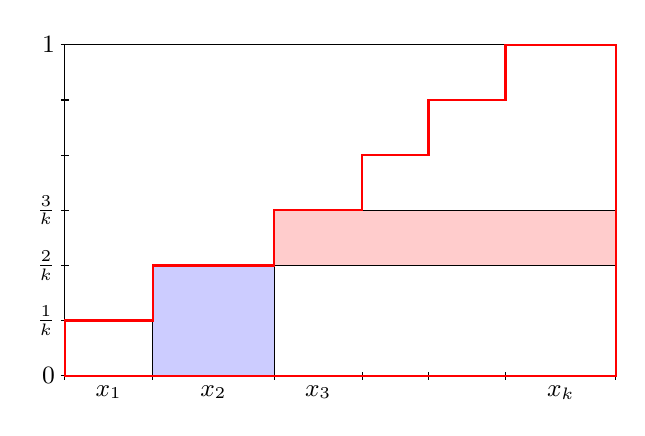
\begin{tikzpicture}[scale=0.7]
		\draw (0,0) rectangle (10,6);

		\foreach \x in {0, 1.6, 3.8, 5.4, 6.6, 8, 10} {\draw (\x,-2pt) -- (\x,2pt);}
		\foreach \y in {0, ..., 6} {\draw (-2pt,\y) -- (2pt,\y);}

		\path (0,0) -- node[below] {\small{$x_1$}} (1.6,0);
		\path (1.6,0) -- node[below] {\small{$x_2$}} (3.8,0);
		\path (3.8,0) -- node[below] {\small{$x_3$}} (5.4,0);
		\path (8,0) -- node[below] {\small{$x_k$}} (10,0);

		\node[left] at (0,0) {\small{$0$}};
		\node[left] at (0,1) {\small{$\frac{1}{k}$}};
		\node[left] at (0,2) {\small{$\frac{2}{k}$}};
		\node[left] at (0,3) {\small{$\frac{3}{k}$}};
		\node[left] at (0,6) {\small{$1$}};
		
		\visible<2->{\filldraw[fill=blue!20,draw=black] (1.6,0) rectangle (3.8,2);}
		\visible<3->{\filldraw[fill=red!20,draw=black] (3.8,2) rectangle (10,3);}

		\draw[red,thick] (0,0) |- (1.6,1) |- (3.8,2) |- (5.4,3) |- (6.6,4) |- (8,5) |- (10,6) |- cycle;
	\end{tikzpicture}
	\flushleft
	\tikz \draw[red,thick] (0,0) rectangle (0.25,0.25);
	\small{Revenue}\\
    \visible<2->{
        \tikz \filldraw[fill=blue!20,draw=black] (0,0) rectangle (0.25,0.25);
        \small{Total money spent by bidders of type $2$}\\
    }
    \visible<3->{
        \tikz \filldraw[fill=red!20,draw=black] (0,0) rectangle (0.25,0.25);
        \small{Total money spent by bidders from slab $3$}
    }
\end{frame}

\begin{frame}
    \frametitle{Assumptions}
	\begin{enumerate}
        \item<1-> $\forall (u,v) \in E: c_{u,v} \leq \frac{1}{k^2}$.
        \item<1-> Each bidder has a budget of $1$.
        \item<1-> \textcolor{orange}{OPT} exhausts the budget of each bidder.
        \item<1-> Each bidder of type $i \in \{1,...,k \}$ spends exactly $\frac{i}{k}$.
        \invisible<1->{\item<1-> All non-zero bids are equal.}
	\end{enumerate}
\end{frame}

\begin{frame}
    \frametitle{Assumptions}
    Each bidder of type $i \in \{1,...,k \}$ spends exactly $\frac{i}{k}$.\\
    \smallskip
    The total error resulting from this simplification is at most $\frac{n}{k}$.\\
    \smallskip
    \centering
    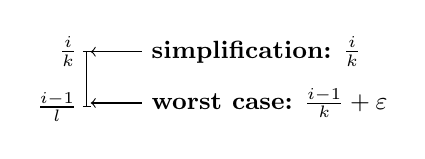
\begin{tikzpicture}[scale=0.7]
        \visible<2->{
            \draw (0,0) -- (0,1);
		
            \draw (-2pt,0) -- (2pt,0);
            \draw (-2pt,1) -- (2pt,1);
    
            \node[left] at (0,0) {\small{$\frac{i-1}{l}$}};
            \node[left] at (0,1) {\small{$\frac{i}{k}$}};
        }
    
        \visible<3->{\draw[->] (1,1) node[right] {\small{\textbf{simplification:} $\frac{i}{k}$}} -- (2pt,1);}
    
        \visible<4->{\draw[->] (1,2pt) node[right] {\small{\textbf{worst case:} $\frac{i-1}{k} + \varepsilon$}} -- (2pt,2pt);}
    \end{tikzpicture}
    \flushleft
    \visible<5->{Error for a bidder of type $i$ is at most: $\frac{i}{k} - \left(\frac{i-1}{k} + \varepsilon \right) = \frac{1}{k} - \varepsilon \leq \frac{1}{k}$\\}
    \smallskip
    \visible<6->{Total error is at most: $n \frac{1}{k} = \frac{n}{k}$}
\end{frame}

\begin{frame}
    \frametitle{Relation Between the $\beta_i$ and $x_i$}
    \centering
    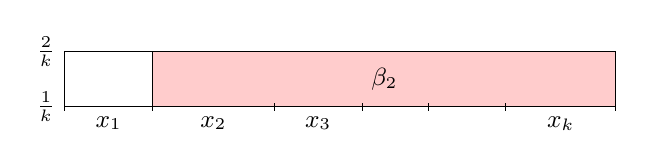
\begin{tikzpicture}[scale=0.7]
		\fill[red!20] (1.6,0) rectangle node[black] {\small{$\beta_2$}} (10,1);

		\draw (0,0) rectangle (10,1);

		\foreach \x in {0, 1.6, 3.8, 5.4, 6.6, 8, 10} {\draw (\x,-2pt) -- (\x,2pt);}

		\path (0,0) -- node[below] {\small{$x_1$}} (1.6,0);
		\path (1.6,0) -- node[below] {\small{$x_2$}} (3.8,0);
		\path (3.8,0) -- node[below] {\small{$x_3$}} (5.4,0);
		\path (8,0) -- node[below] {\small{$x_k$}} (10,0);

		\node[left] at (0,0) {\small{$\frac{1}{k}$}};
		\node[left] at (0,1) {\small{$\frac{2}{k}$}};
		
		\draw (1.6,0) -- (1.6,1);
	\end{tikzpicture}\\
	\small{$=$}\\
	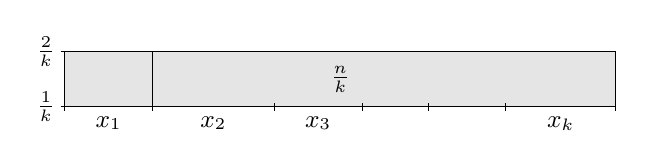
\begin{tikzpicture}[scale=0.7]
		\filldraw[fill=gray!20] (0,0) rectangle node {\small{$\frac{n}{k}$}} (10,1);
		
		\foreach \x in {0, 1.6, 3.8, 5.4, 6.6, 8, 10} {\draw (\x,-2pt) -- (\x,2pt);}

		\draw (-2pt,0) -- (2pt,0);
		\draw (-2pt,1) -- (2pt,1);

		\path (0,0) -- node[below] {\small{$x_1$}} (1.6,0);
		\path (1.6,0) -- node[below] {\small{$x_2$}} (3.8,0);
		\path (3.8,0) -- node[below] {\small{$x_3$}} (5.4,0);
		\path (8,0) -- node[below] {\small{$x_k$}} (10,0);

		\node[left] at (0,0) {\small{$\frac{1}{k}$}};
		\node[left] at (0,1) {\small{$\frac{2}{k}$}};
		
		\draw (1.6,0) -- (1.6,1);
	\end{tikzpicture}\\
	\small{$-$}\\
	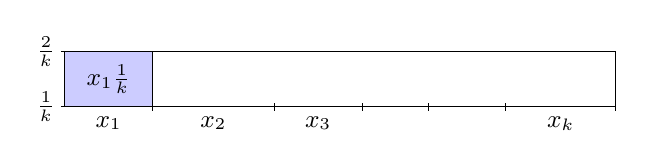
\begin{tikzpicture}[scale=0.7]
		\fill[blue!20] (0,0) rectangle node[black] {\small{$x_1 \frac{1}{k}$}} (1.6,1);
		
		\draw (0,0) rectangle (10,1);

		\draw (1.6,-2pt) -- (1.6,2pt);
		\draw (3.8,-2pt) -- (3.8,2pt);
		\draw (5.4,-2pt) -- (5.4,2pt);
		\draw (6.6,-2pt) -- (6.6,2pt);

		\draw (8,-2pt) -- (8,2pt);
		\draw (10,-2pt) -- (10,2pt);
		\draw (-2pt,0) -- (2pt,0);
		\draw (-2pt,1) -- (2pt,1);

		\path (0,0) -- node[below] {\small{$x_1$}} (1.6,0);
		\path (1.6,0) -- node[below] {\small{$x_2$}} (3.8,0);
		\path (3.8,0) -- node[below] {\small{$x_3$}} (5.4,0);
		\path (8,0) -- node[below] {\small{$x_k$}} (10,0);

		\node[left] at (0,0) {\small{$\frac{1}{k}$}};
		\node[left] at (0,1) {\small{$\frac{2}{k}$}};
		
		\draw (1.6,0) -- (1.6,1);
    \end{tikzpicture}
    \begin{equation*}
        \forall i \in \{1, \dots, k \}: \beta_i = \frac{n - \sum_{j=1}^{i-1} x_j}{k}
    \end{equation*}
\end{frame}

\begin{frame}
    \frametitle{Revenue Calculation for MSVV via Types}
    \centering
    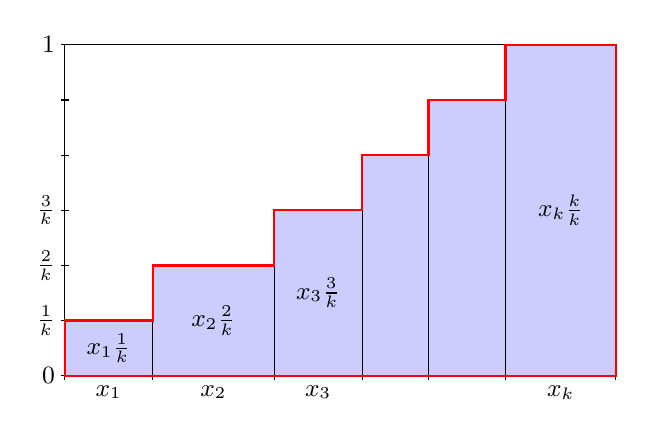
\begin{tikzpicture}[scale=0.7]
		\draw (0,0) rectangle (10,6);

		\foreach \x in {0, 1.6, 3.8, 5.4, 6.6, 8, 10} {\draw (\x,-2pt) -- (\x,2pt);}
		\foreach \y in {0, ..., 6} {\draw (-2pt,\y) -- (2pt,\y);}

		\path (0,0) -- node[below] {\small{$x_1$}} (1.6,0);
		\path (1.6,0) -- node[below] {\small{$x_2$}} (3.8,0);
		\path (3.8,0) -- node[below] {\small{$x_3$}} (5.4,0);
		\path (8,0) -- node[below] {\small{$x_k$}} (10,0);

		\node[left] at (0,0) {\small{$0$}};
		\node[left] at (0,1) {\small{$\frac{1}{k}$}};
		\node[left] at (0,2) {\small{$\frac{2}{k}$}};
		\node[left] at (0,3) {\small{$\frac{3}{k}$}};
		\node[left] at (0,6) {\small{$1$}};
		
		\filldraw[fill=blue!20,draw=black] (0,0) rectangle node {\small{$x_1 \frac{1}{k}$}} (1.6,1);
		\filldraw[fill=blue!20,draw=black] (1.6,0) rectangle node {\small{$x_2 \frac{2}{k}$}} (3.8,2);
		\filldraw[fill=blue!20,draw=black] (3.8,0) rectangle node {\small{$x_3 \frac{3}{k}$}} (5.4,3);
		\filldraw[fill=blue!20,draw=black] (5.4,0) rectangle (6.6,4);
		\filldraw[fill=blue!20,draw=black] (6.6,0) rectangle (8,5);
		\filldraw[fill=blue!20,draw=black] (8,0) rectangle node {\small{$x_k \frac{k}{k}$}} (10,6);

		\draw[red,thick] (0,0) |- (1.6,1) |- (3.8,2) |- (5.4,3) |- (6.6,4) |- (8,5) |- (10,6) |- cycle;
    \end{tikzpicture}
    \visible<2->{
        \begin{equation*}
            \pi_{\text{\textcolor{orange}{MSVV}}} \geq \sum_{i=1}^k x_i \frac{i}{k} - \frac{n}{k}
        \end{equation*}
    }
\end{frame}

\begin{frame}
    \frametitle{Revenue Calculation for MSVV via Slabs}
    \centering
    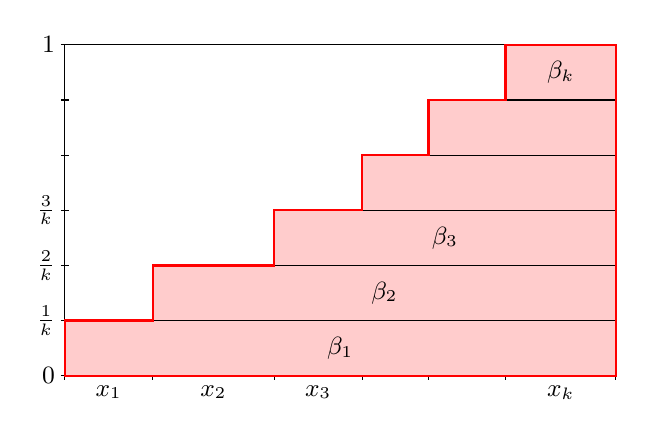
\begin{tikzpicture}[scale=0.7]
		\draw (0,0) rectangle (10,6);

		\foreach \x in {0, 1.6, 3.8, 5.4, 6.6, 8, 10} {\draw (\x,-2pt) -- (\x,2pt);}
		\foreach \y in {0, ..., 6} {\draw (-2pt,\y) -- (2pt,\y);}

		\path (0,0) -- node[below] {\small{$x_1$}} (1.6,0);
		\path (1.6,0) -- node[below] {\small{$x_2$}} (3.8,0);
		\path (3.8,0) -- node[below] {\small{$x_3$}} (5.4,0);
		\path (8,0) -- node[below] {\small{$x_k$}} (10,0);

		\node[left] at (0,0) {\small{$0$}};
		\node[left] at (0,1) {\small{$\frac{1}{k}$}};
		\node[left] at (0,2) {\small{$\frac{2}{k}$}};
		\node[left] at (0,3) {\small{$\frac{3}{k}$}};
		\node[left] at (0,6) {\small{$1$}};
		
		\filldraw[fill=red!20,draw=black] (0,0) rectangle node {\small{$\beta_1$}} (10,1);
		\filldraw[fill=red!20,draw=black] (1.6,1) rectangle node {\small{$\beta_2$}} (10,2);
		\filldraw[fill=red!20,draw=black] (3.8,2) rectangle node {\small{$\beta_3$}} (10,3);
		\filldraw[fill=red!20,draw=black] (5.4,3) rectangle (10,4);
		\filldraw[fill=red!20,draw=black] (6.6,4) rectangle (10,5);
		\filldraw[fill=red!20,draw=black] (8,5) rectangle node {\small{$\beta_k$}} (10,6);

		\draw[red,thick] (0,0) |- (1.6,1) |- (3.8,2) |- (5.4,3) |- (6.6,4) |- (8,5) |- (10,6) |- cycle;
    \end{tikzpicture}
    \visible<2->{
        \begin{equation*}
            \pi_{\text{\textcolor{orange}{MSVV}}} \geq \sum_{i=1}^k \beta_i - \frac{n}{k}
        \end{equation*}
    }
\end{frame}

%\section*{Optimization Problems}

\begin{frame}
    \frametitle{Optimization Problem}
    \begin{definition}
        An instance of an \alert{optimization problem} is specified by the data:
        \begin{equation*}
            n \in \mathbb{N}
            \visible<2->{, \qquad F \subseteq \mathbb{R}^n}
            \visible<3->{, \qquad \varphi: \mathbb{R}^n \to \mathbb{R}}
            \visible<4->{, \qquad \text{opt} \in \{\min, \max \}}
        \end{equation*}
        \visible<5->{%
            A point $x^* \in F$ is \alert{optimal} if
            \begin{align*}
                x \in F \quad \Rightarrow \quad \varphi(x^*) \leq \varphi(x) \qquad & \text{for} \; \text{opt} = \min \\
                x \in F \quad \Rightarrow \quad \varphi(x^*) \geq \varphi(x) \qquad & \text{for} \; \text{opt} = \max
            \end{align*}
        }%
        \visible<6->{\textbf{Goal:} Optimize $\varphi$ over $F$, i.e., decide if $F = \emptyset$, or find an optimal point $x^*$, or decide that $\varphi$ is not bounded from below ($\text{opt} = \min$) or above ($\text{opt} = \max$).}
    \end{definition}
\end{frame}

\begin{frame}
    \frametitle{Linear Optimization Problem}
    \begin{definition}
        An instance of a \alert{linear optimization problem} or a \alert{linear program (LP)} is specified by the data:
        \begin{equation*}
            m, n \in \mathbb{N}
            \visible<2->{, \quad a_1, \dots, a_m \in \mathbb{R}^n}
            \visible<3->{, \quad \beta_1, \dots, \beta_m \in \mathbb{R}}
            \visible<4->{, \quad \gamma_1, \dots, \gamma_n \in \mathbb{R}}
        \end{equation*}
        \visible<5->{%
            The linear functional $\varphi: \mathbb{R}^n \rightarrow \mathbb{R}$ for $x := (\xi_1, \dots, \xi_n)^T \in \mathbb{R}$ is defined by
            $$\varphi(x) := \sum_{i=1}^n \gamma_i \xi_i$$
            and let
            $$F := \{x \in \mathbb{R}^n: a_1^T x \leq \beta_1 \; \land \; \dots \; \land \; a_m^T x \leq \beta_m \}$$    
        }%
        \visible<6->{\textbf{Goal:} \textcolor{blue}{Maximize} $\varphi$ over $F$.}
    \end{definition}
\end{frame}

\begin{frame}
    \frametitle{Linear Optimization Problem}
    \begin{block}{Notation}
        Let $(m, n, a_1, \dots, a_m, \beta_1, \dots, \beta_m, \gamma_1, \dots, \gamma_n)$ be an instance of a linear optimization problem.
        Set
        \begin{alignat*}{2}
            A & := (a_1, \dots, a_m)^T & & \in \mathbb{R}^{m \times n} \\
            b & := (\beta_1, \dots, \beta_m)^T & & \in \mathbb{R}^m \\
            c & := (\gamma_1, \dots, \gamma_n)^T & & \in \mathbb{R}^n
        \end{alignat*}
        Then we often write
        \begin{gather*}
            \max \; c^T x \\
            Ax \leq b
        \end{gather*}
    \end{block}
\end{frame}

\subsection{Special Case: BALANCE for $b$-Matching}

\begin{frame}
    \frametitle{Assumptions}
	\begin{enumerate}
        \item<1-> $\forall (u,v) \in E: c_{u,v} \leq \frac{1}{k^2}$.
        \item<1-> Each bidder has a budget of $1$.
        \item<1-> \textcolor{orange}{OPT} exhausts the budget of each bidder.
        \item<1-> Each bidder of type $i \in \{1,...,k \}$ spends exactly $\frac{i}{k}$.
        \item<1-> All non-zero bids are equal.
	\end{enumerate}
\end{frame}

\begin{frame}
    \frametitle{Landscape of Problems}
    \centering
    \begin{tikzpicture}
        \begin{scope}
            \clip \greenellipse;
            \fill[gray!25] \blueellipse;
        \end{scope}
        \draw[very thick,orange] \orangeellipse;
        \draw[very thick,blue] \blueellipse;
		\draw[very thick,violet] \violetellipse;
		\draw[very thick,green!70!black] \greenellipse;
		\draw[very thick,red] \redellipse;
	\end{tikzpicture}
\end{frame}

\begin{frame}
    \frametitle{A Linear Program for BALANCE}
    \begin{lemma}
        Let $v \in V$. If \textcolor{orange}{OPT} assigns query $v$ to a bidder of type $i \in \{1, \dots, k-1 \}$, then \textcolor{orange}{Balance} gets the money for $v$ from some slab $j$ such that $1 \leq j \leq i$.
    \end{lemma}
    \begin{lemma}
        \begin{equation*}
            \forall i \in \{1, \dots, k-1 \}: \sum_{j=1}^i x_j \leq \sum_{j=1}^i \beta_i
        \end{equation*}
    \end{lemma}
\end{frame}

\begin{frame}
    \frametitle{Revenue Calculation for OPT}
    \centering
    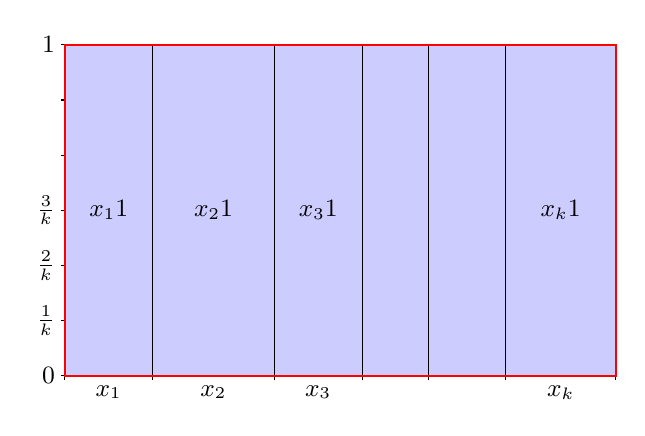
\begin{tikzpicture}[scale=0.7]
		\draw (0,0) rectangle (10,6);

		\foreach \x in {0, 1.6, 3.8, 5.4, 6.6, 8, 10} {\draw (\x,-2pt) -- (\x,2pt);}
		\foreach \y in {0, ..., 6} {\draw (-2pt,\y) -- (2pt,\y);}

		\path (0,0) -- node[below] {\small{$x_1$}} (1.6,0);
		\path (1.6,0) -- node[below] {\small{$x_2$}} (3.8,0);
		\path (3.8,0) -- node[below] {\small{$x_3$}} (5.4,0);
		\path (8,0) -- node[below] {\small{$x_k$}} (10,0);

		\node[left] at (0,0) {\small{$0$}};
		\node[left] at (0,1) {\small{$\frac{1}{k}$}};
		\node[left] at (0,2) {\small{$\frac{2}{k}$}};
		\node[left] at (0,3) {\small{$\frac{3}{k}$}};
		\node[left] at (0,6) {\small{$1$}};
		
		\filldraw[fill=blue!20,draw=black] (0,0) rectangle node {\small{$x_1 1$}} (1.6,6);
		\filldraw[fill=blue!20,draw=black] (1.6,0) rectangle node {\small{$x_2 1$}} (3.8,6);
		\filldraw[fill=blue!20,draw=black] (3.8,0) rectangle node {\small{$x_3 1$}} (5.4,6);
		\filldraw[fill=blue!20,draw=black] (5.4,0) rectangle (6.6,6);
		\filldraw[fill=blue!20,draw=black] (6.6,0) rectangle (8,6);
		\filldraw[fill=blue!20,draw=black] (8,0) rectangle node {\small{$x_k 1$}} (10,6);

		\draw[red,thick] (0,0) rectangle (10,6);
    \end{tikzpicture}
    \visible<2->{
        \begin{equation*}
            \pi_{\text{\textcolor{orange}{OPT}}} = \sum_{i=1}^k x_i = n
        \end{equation*}
    }
\end{frame}

\begin{frame}
    \frametitle{A Linear Program for BALANCE}
    \begin{lemma}
        \begin{equation*}
            \forall i \in \{1, \dots, k-1 \}: \sum_{j=1}^i \left(1 + \frac{i-j}{k} \right) x_j \leq \frac{i}{k} n
        \end{equation*}
    \end{lemma}
\end{frame}

\begin{frame}
    \frametitle{A Linear Program for BALANCE}
    \begin{align*}
		\visible<1->{\pi_{\text{\textcolor{orange}{BALANCE}}} & \geq \sum_{i=1}^{\textcolor<2>{blue}{k}} x_i \frac{i}{k} - \frac{n}{k}}\\
		\visible<2->{& = \sum_{i=1}^{\textcolor<2>{blue}{k-1}} \frac{i}{k} x_i + \textcolor<2,3>{blue}{x_k} - \frac{n}{k}}\\
		\visible<3->{& = \textcolor<4>{blue}{\sum_{i=1}^{k-1} \frac{i}{k} x_i} + \textcolor<3>{blue}{\left(n \textcolor<4>{blue}{- \sum_{i=1}^{k-1} x_i} \right)} - \frac{n}{k}}\\
		\visible<4->{& = n \textcolor<4>{blue}{- \sum_{i=1}^{k-1} \textcolor<5>{blue}{\left(1 - \frac{i}{k} \right)} x_i} - \frac{n}{k}}\\
		\visible<5->{& = n - \sum_{i=1}^{k-1} \textcolor<5>{blue}{\frac{k-i}{k}} x_i - \frac{n}{k}}
	\end{align*}
\end{frame}

\begin{frame}
    \frametitle{A Linear Program for BALANCE}
    \begin{block}{Notation}
        The linear program \textcolor{orange}{(P)} is defined by
        \begin{align*}
            \text{maximize} \quad & \sum_{i=1}^{k-1} \frac{k-i}{k} x_i \\
            \text{subject to} \quad &
            \begin{aligned}[t]
                \sum_{j=1}^i \left(1 + \frac{i-j}{k} \right) x_j & \leq \frac{i}{k} n & \forall i \in \{1, \dots, k-1\} \\
                x_i & \geq 0 & \forall i \in \{1, \dots, k-1\}
            \end{aligned}
        \end{align*}
    \end{block}
\end{frame}

%\section*{Duality}

\begin{frame}
    \frametitle{Duality}
    \begin{block}{Notation}
        The two linear programs \text{\textcolor{orange}{(I)}} and \text{\textcolor{orange}{(II)}} are defined by
        \begin{equation*}
            \text{\textcolor{orange}{(I)}} \quad
            \begin{gathered}
                \max \; c^T x \\
                \begin{aligned}
                    Ax & \leq b \\
                    x & \geq 0
                \end{aligned}
            \end{gathered}
            \qquad \qquad
            \text{\textcolor{orange}{(II)}} \quad
            \begin{gathered}
                \min \; b^T y \\
                \begin{aligned}
                    A^T y & \geq c \\
                    y & \geq 0
                \end{aligned}
            \end{gathered}
        \end{equation*}
        Let
        \begin{align*}
            P & := \{x \in \mathbb{R}^n: Ax \leq b \; \land \; x \geq 0 \} \\
            Q & := \{y \in \mathbb{R}^m: A^T y \geq c \; \land \; y \geq 0 \}
        \end{align*}
        and $\zeta_{\text{\textcolor{orange}{(I)}}}$, $\zeta_{\text{\textcolor{orange}{(II)}}}$ be the optimum values of \text{\textcolor{orange}{(I)}}, \text{\textcolor{orange}{(II)}} respectively.
    \end{block}
\end{frame}

\begin{frame}
    \frametitle{Duality}
    \begin{definition}
        The linear programs \text{\textcolor{orange}{(I)}} and \text{\textcolor{orange}{(II)}} are called \alert{dual} of each other. Often one is called \alert{primal}, the other \alert{dual}.
    \end{definition}
\end{frame}

\begin{frame}
    \frametitle{Duality}
    \begin{theorem}
        The following statements hold:
        \begin{enumerate}
            \item $\zeta_{\text{\textcolor{orange}{(I)}}} \leq \zeta_{\text{\textcolor{orange}{(II)}}}$
            \item $P \neq \emptyset \; \lor \; Q \neq \emptyset \quad \Rightarrow \quad \zeta_{\text{\textcolor{orange}{(I)}}} = \zeta_{\text{\textcolor{orange}{(II)}}}$
            \item \label{thm:duality} Let $x^* \in P, y^* \in Q$. Then
            \begin{align*}
                & c^T x^* = b^T y^* \\
                \iff & \zeta_{\text{\textcolor{orange}{(I)}}} = c^T x^* \; \land \; \zeta_{\text{\textcolor{orange}{(II)}}} = b^T y^* \\
                \iff & (y^*)^T \left(b - Ax^* \right) = 0 \; \land \; (x^*)^T \left(c - A^T y^* \right) = 0
            \end{align*}
        \end{enumerate}
    \end{theorem}
\end{frame}

\begin{frame}
    \frametitle{A Solution to the Linear Program}
    \begin{block}{Notation}
        The dual linear program of \textcolor{orange}{(P)}, \textcolor{orange}{(D)}, is defined by
        \begin{align*}
            \text{minimize} \quad & \sum_{i=1}^{k-1} \frac{i}{k} n y_i \\
            \text{subject to} \quad &
            \begin{aligned}[t]
                \sum_{j=i}^{k-1} \left(1 + \frac{j-i}{k} \right) y_j & \geq \frac{k-i}{k} & \forall i \in \{1, \dots, k-1 \} \\
                y_i & \geq 0 & \forall i \in \{1, \dots, k-1 \}
            \end{aligned}
        \end{align*}
    \end{block}
\end{frame}

\begin{frame}
    \frametitle{A Solution to the Linear Program}
    \begin{lemma}
        \begin{equation*}
            x_i^* = \frac{n}{k} \left(1 - \frac{1}{k} \right)^{i-1} \quad \text{for} \; i=1, \dots, k-1
        \end{equation*}
        is a solution to the system
        \begin{equation*}
            \sum_{j=1}^i \left(1 + \frac{i-j}{k} \right) x_j = \frac{i}{k} n \quad \forall i \in \{1, \dots, k-1 \}
        \end{equation*}
    \end{lemma}
\end{frame}

\begin{frame}
    \frametitle{A Solution to the Linear Program}
    \begin{lemma}
        \begin{equation*}
            y_i^* = \frac{1}{k} \left(1 - \frac{1}{k} \right)^{k-i-1} \quad \text{for} \; i=1, \dots, k-1
        \end{equation*}
        is a solution to the system
        \begin{equation*}
            \sum_{j=i}^{k-1} \left(1 + \frac{j-i}{k} \right) y_j = \frac{k-i}{k} \quad \forall i \in \{1, \dots, k-1 \}
        \end{equation*}
    \end{lemma}
\end{frame}

\begin{frame}
    \frametitle{A Solution to the Linear Program}
    \begin{lemma}
        The optimum objective function value of the LP \textcolor{orange}{(P)} is $n \left(1 - \frac{1}{k} \right)^k$.
    \end{lemma}
    \begin{proof}
        \let\qed\relax
        \begin{equation*}
            x_i^* = \frac{n}{k} \left(1 - \frac{1}{k} \right)^{i-1} \quad \text{for} \; i=1, \dots, k-1
        \end{equation*}
        and
        \begin{equation*}
            y_i^* = \frac{1}{k} \left(1 - \frac{1}{k} \right)^{k-i-1} \quad \text{for} \; i=1, \dots, k-1
        \end{equation*}
        are \textcolor{blue}{feasible} solutions of the primal and dual programs.
    \end{proof}
\end{frame}

\begin{frame}
	\frametitle{A Solution to the Linear Program}
	\begin{proof}[Proof (continued)]
		By construction, they clearly satisfy
		\begin{align*}
			(y^*)^T \left(b - Ax^* \right) = 0 \; \land \; (x^*)^T \left(c - A^T y^* \right) = 0
		\end{align*}
		\visible<2->{Hence, they are also \textcolor{blue}{optimum} solutions of the primal and dual programs.\\}
		\smallskip
		\visible<3->{This gives an optimum objective function value of}
		\begin{equation*}
			\visible<3->{c^T x^* = \sum_{i=1}^{k-1} \frac{k-i}{k} \frac{n}{k} \left(1 - \frac{1}{k} \right)^{i-1}}
			\visible<4->{= n \left(1 - \frac{1}{k} \right)^k}
        \end{equation*}
        \visible<4->{\qedhere}
	\end{proof}
\end{frame}

\begin{frame}No randomized online algorithm can have a competitive ratio better than $1 - \frac{1}{e}$ for the $b$-Matching problem, for large $b$.
    \frametitle{Competitive Ratio of BALANCE for $b$-Matching}
    \begin{theorem}
        \textcolor{orange}{BALANCE} achieves a competitive ratio of $1 - \frac{1}{e}$ for the $b$-Matching problem, for large $b$.
    \end{theorem}
    \begin{theorem}
        No \textcolor{blue}{randomized} online algorithm can have a competitive ratio better than $1 - \frac{1}{e}$ for the $b$-Matching problem, for large $b$.
    \end{theorem}
\end{frame}

\subsection{General Case: MSVV for Adwords with Small Bids}

\begin{frame}
    \frametitle{Assumptions}
	\begin{enumerate}
        \item<1-> Each bid is small compared to the corresponding budget \mbox{(i.e., $\forall (u,v) \in E: c_{u,v} \ll b_u$}).
        \item<1-> Each bidder has a budget of $1$.
        \item<1-> \textcolor{orange}{OPT} exhausts the budget of each bidder.
        \item<1-> Each bidder of type $i \in \{1,...,k \}$ spends exactly $\frac{i}{k}$.
        \item<1-> \sout{All non-zero bids are equal.}
	\end{enumerate}
\end{frame}

\begin{frame}
    \frametitle{Landscape of Problems}
    \centering
    \begin{tikzpicture}
        \fill[gray!25] \blueellipse;
        \draw[very thick,orange] \orangeellipse;
        \draw[very thick,blue] \blueellipse;
		\draw[very thick,violet] \violetellipse;
		\draw[very thick,green!70!black] \greenellipse;
		\draw[very thick,red] \redellipse;
	\end{tikzpicture}
\end{frame}

\begin{frame}
    \frametitle{An Inequality Constraint for MSVV}
    \begin{block}{Notation}
        Let \textcolor{orange}{ALG} $\in \{\text{\textcolor{orange}{OPT}}, \text{\textcolor{orange}{MSVV}} \}, v \in V$. Then $u_{\text{\textcolor{orange}{ALG}}}(v)$ denotes the bidder \textcolor{orange}{ALG} assigns query $v$ to.
    \end{block}
    \begin{lemma}
        For all queries$v \in V$ such that $\text{type}(u_{\text{\textcolor{orange}{OPT}}}(v)) \in \{1, \dots, k-1 \}:$
        \begin{equation*}
            c_{u_{\text{\textcolor{orange}{OPT}}}(v),v} \psi_k \left(\text{type}(u_{\text{\textcolor{orange}{OPT}}}(v) \right) \leq c_{u_{\text{\textcolor{orange}{MSVV}}}(v),v} \psi_k \left(\text{slab}(u_{\text{\textcolor{orange}{MSVV}}}(v) \right)
        \end{equation*}
    \end{lemma}
\end{frame}

\begin{frame}
    \frametitle{An Inequality Constraint for MSVV}
    \begin{lemma}
        \begin{equation*}
            \sum_{i=1}^{k-1} \psi_k(i) x_i \leq \sum_{i=1}^{k-1} \psi_k(i) \beta_i + \frac{n}{k}
        \end{equation*}
    \end{lemma}
\end{frame}

\begin{frame}
    \frametitle{Competitive Ratio for MSVV for Adwords with Small Bids}
    \begin{theorem}
        \textcolor{orange}{MSVV} achieves a competitive ratio of $1 - \frac{1}{e}$ for the Adwords problem with small bids.
    \end{theorem}
\end{frame}

\begin{frame}
    \frametitle{Competitive Ratio for MSVV for Adwords with Small Bids}
    \begin{proof}
        \let\qed\relax
        We can use
        \begin{equation*}
            \forall i \in \{1, \dots, k \}: \beta_i = \frac{n - \sum_{j=1}^{i-1} x_j}{k}
        \end{equation*}
        and the explicit form of the perturbation function $\varphi(x) = 1 - e^{x-1}$ in
        \begin{equation*}
            \sum_{i=1}^{k-1} \psi_k(i) x_i \leq \sum_{i=1}^{k-1} \psi_k(i) \beta_i + \frac{n}{k}
        \end{equation*}
    \end{proof}
\end{frame}

\begin{frame}
    \frametitle{Competitive Ratio for MSVV for Adwords with Small Bids}
    \begin{proof}[Proof (continued)]
        to get
        \begin{equation*}
            \sum_{i=1}^k x_i \frac{i}{k} - \frac{n}{k} \geq n \left(1 - \frac{1}{e} \right), \quad \text{as} \; k \to \infty
        \end{equation*}
        But the left hand side is a lower bound on $\pi_{\text{\textcolor{orange}{MSVV}}}$, thus proving the theorem.
    \end{proof}
\end{frame}